\documentclass[tikz,border=5pt]{standalone}
\usepackage{pgfplots}
\usetikzlibrary{arrows.meta}
\pgfplotsset{compat=1.18}

\definecolor{corba}{HTML}{365FB3}
\definecolor{punt}{HTML}{C2415D}
\definecolor{guia}{HTML}{6B7280}

\begin{document}
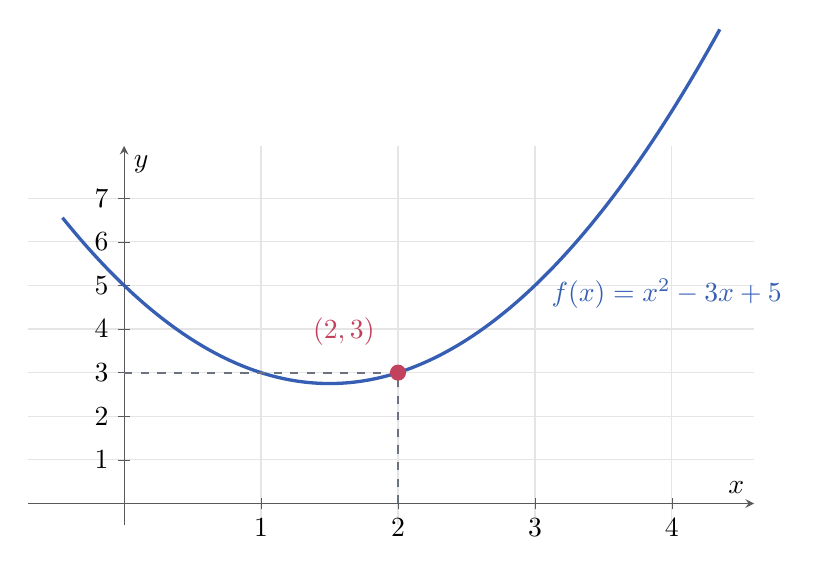
\begin{tikzpicture}
  \begin{axis}[
    width=10.8cm,
    height=6.4cm,
    axis lines=middle,
    xmin=-0.7,
    xmax=4.6,
    ymin=-0.5,
    ymax=8.2,
    xlabel={$x$},
    ylabel={$y$},
    xtick={1,2,3,4},
    ytick={1,2,3,4,5,6,7},
    axis line style={black!65},
    tick style={black!65},
    grid=major,
    grid style={black!10},
    clip=false,
  ]
    \addplot[corba, very thick, domain=-0.45:4.35, samples=180]
      {x^2-3*x+5};

    \addplot[guia, dashed, thick] coordinates {(2,0) (2,3)};
    \addplot[guia, dashed, thick] coordinates {(0,3) (2,3)};
    \addplot[only marks, mark=*, mark size=2.7pt, punt]
      coordinates {(2,3)};

    \node[anchor=south west, text=corba]
      at (axis cs:3.05,4.25) {$f(x)=x^2-3x+5$};
    \node[anchor=south east, text=punt]
      at (axis cs:1.9,3.4) {$(2,3)$};
  \end{axis}
\end{tikzpicture}
\end{document}
